\documentclass[../../main.tex]{subfiles}
\begin{document}

\begin{flushright}
\footnotesize\textit{【自動文字起こし・要確認】}
\end{flushright}

{\bf [解]} $P$ から $\alpha$ に下ろした垂足を $H$ とし，$PH = h$ とおく．又，球の中心を $O$ とする．$O, P$ を含む平面で切ると，対称性から右下図のようになる．ここで，$O$ を原点，$OP$ を $x$ 軸正方向とする $xy$ 平面を定める．右図のように $\theta$ を定める ($0 < \theta < \pi/2$)．又以下，$c = \cos\theta, s = \sin\theta$ とする．$P$ は，円の接線 $cx + sy = 1$ と $x$ 軸の交点で，$P\left(\dfrac{1}{c}, 0\right)$ となる．したがって
\begin{align}
h = \dfrac{1}{c} - c \quad \dots \text{①}
\end{align}
であり，$D$ は斜線部分を $x$ 軸まわりに回転したもので，体積 $V_D$ として
\begin{align}
V_D &= \dfrac{1}{3} \cdot \pi s^2 \cdot h - \pi \int_c^1 (1-x^2) \, dx \\
&= \dfrac{1}{3} \pi s^2 \Bigl(\dfrac{1}{c} - c\Bigr) - \pi \Bigl[ \dfrac{2}{3} - c + \dfrac{1}{3} c^3 \Bigr] \quad (\because \text{①}) \\
&= \dfrac{1}{3} \pi \Bigl[ \dfrac{s^2(1-c^2)}{c} + 3c - c^3 - 2 \Bigr] \\
&= \dfrac{1}{3}\pi \dfrac{c^2-2c+1}{c} \quad \dots \text{②}
\end{align}
これが球の体積の $\dfrac{1}{2}$ 倍にひとしいので，
\begin{align}
& V_D = \dfrac{2}{3}\pi \\
\iff &\dfrac{c^2-2c+1}{c} = 2 \\
\iff &c = 2 - \sqrt{3} \quad (\because 0 < c < 1) \quad \dots \text{③}
\end{align}
となる．この時，$K$ の体積 $V_K$ は
\begin{align}
V_K &= \int_c^1 (1-x^2) \cdot \pi \, dx \\
&= \dfrac{2}{3}\pi \Bigl(11 - 6\sqrt{3}\Bigr) \quad (\because \text{③})
\end{align}

\begin{figure}[htb]
\centering
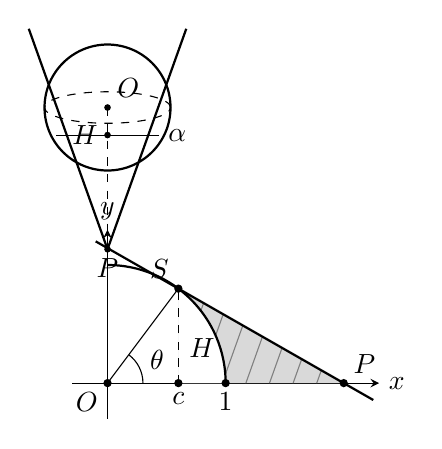
\begin{tikzpicture}[scale=1.0, >=stealth]
  % Upper 3D/2D cone figure
  \begin{scope}[shift={(0,3.5)}]
    \draw[thick] (0,-1.8) -- (-1.0,1.0);
    \draw[thick] (0,-1.8) -- (1.0,1.0);
    \draw[thick] (0,0) circle (0.8);
    \draw[dashed] (0,0) ellipse (0.8 and 0.2);
    \draw (-0.65,-0.35) -- (0.65,-0.35) node[right] {$\alpha$};
    \draw[dashed] (0,0) -- (0,-1.8);
    \fill (0,0) circle (1.2pt) node[above right] {$O$};
    \fill (0,-0.35) circle (1.2pt) node[left] {$H$};
    \fill (0,-1.8) circle (1.2pt) node[below] {$P$};
  \end{scope}

  % Lower 2D coordinate diagram
  \begin{scope}[scale=1.5]
    % Axes
    \draw[->] (-0.3,0) -- (2.3,0) node[right] {$x$};
    \draw[->] (0,-0.3) -- (0,1.3) node[above] {$y$};
    \node[below left] at (0,0) {$O$};

    % Shaded region D
    % Fill between vertical line x=c, line SP, x-axis, and arc
    \begin{scope}
      \clip (0.6,0) -- (0.6,0.8) -- (2.0,0) -- cycle;
      \fill[gray!30] (0.6,0) -- (0.6,0.8) -- (2.0,0) -- cycle;
      \fill[white] (0,0) circle (1.0);
    \end{scope}
    % Hatch lines in shaded region
    \begin{scope}
      \clip (0.6,0) -- (0.6,0.8) -- (2.0,0) -- cycle;
      \clip (0,0) circle (1.0) (2,2) -- (2,-2) -- (-2,-2) -- (-2,2) -- cycle;
      \foreach \x in {0.5, 0.7, ..., 2.2} {
        \draw[gray] (\x, -0.2) -- (\x+0.5, 1.2);
      }
    \end{scope}

    % Circle arc
    \draw[thick] (0,1) arc (90:0:1);

    % Tangent line SP: S=(0.6, 0.8), P=(2.0, 0)
    \draw[thick] (-0.1, 1.2) -- (2.25, -0.143);

    % Vertical line x = c
    \draw[dashed] (0.6,0) -- (0.6,0.8);

    % Line OS
    \draw (0,0) -- (0.6,0.8);

    % Angle theta
    \draw (0.3,0) arc (0:53.13:0.3);
    \node at (0.42,0.2) {$\theta$};

    % Points and labels
    \fill (0,0) circle (1pt);
    \fill (0.6,0.8) circle (1pt) node[above left] {$S$};
    \fill (2.0,0) circle (1pt) node[above right] {$P$};
    \fill (0.6,0) circle (1pt) node[below] {$c$};
    \fill (1,0) circle (1pt) node[below] {$1$};
    \node at (0.8,0.3) {$H$};
  \end{scope}
\end{tikzpicture}
\caption{切り口の3次元図と$xy$平面上の断面図}
\end{figure}

\end{document}
